\documentclass{article}
\usepackage{fullpage,abstract,hyperref,graphicx,caption}
\usepackage{amsmath,amsfonts,amssymb,amsthm,program,float}

\makeatletter

\newfloat{algorithm}{thp}{lop}
\floatname{algorithm}{Algorithm}

\title{
\vspace{-60pt}
CS 6491 - Project 1 - Packing Game
\vspace{-20pt}
}
\date{}

\newcommand\photo[3]{
  \centering
  \includegraphics[width=80pt]{../team/#1}
  \\\textbf{#2}\\[2pt]\texttt{\small#3}\\[5pt]
}

\newcommand\screenshot[1]{\includegraphics[scale=0.15]{#1}}

\begin{document}

\makeatletter
\twocolumn[
\begin{@twocolumnfalse}
\maketitle
{\centering\begin{tabular}{
  p{0.2\textwidth}p{0.2\textwidth}p{0.2\textwidth}p{0.2\textwidth}}
\photo{anshul}{Anshul Bhatnagar}{anshul.bhatnagar\\@gatech.edu} &
\photo{gaurav}{Gaurav Dhage}{gr8dhage\\@gmail.com} &
\photo{chris}{Chris Martin}{chris.martin\\@gatech.edu} &
\photo{suraj}{Suraj Sirpilli}{surajsirpilli\\@gatech.edu}
\end{tabular}

}

\begin{abstract}

We implemented a two-player game in which players arrange a collection
of non-overlapping disks on a plane.
The objective is to minimize the size of the smallest circle
that encloses all of the disks.
The field of play is set up with two identical sets of disks so
game can be played between two humans or against the computer.

\end{abstract}
\end{@twocolumnfalse}
]
\makeatother

\begin{figure}
\centering
\screenshot{init}
\caption{A game's starting configuration.}
\end{figure}

\begin{figure}
\centering
\screenshot{end}
\caption{A human's best attempt (left)
  and our packing algorithm (right).}
\end{figure}

\section{Collision detection}

The game rules disallow overlapping disks, and we want to make
an interface that allows a player to easily position disks
directly adjacent to one another.
So when a mouse drag attempts to move a disk to a location that
would cause overlap, we instead move the disk to the nearest
valid location, as illustrated by Figure \ref{fig:drag}.

When a disk is being moved, we model the situation as a point
being moved among disks that are expanded by the radius of the
moving disk.
If the point is inside any of the expanded disks, this indicates
overlap and therefore an invalid position.

There are two collision resolving methods, both of which
are depicted in Figure \ref{fig:expand}:

\begin{enumerate}
\item If the point intersects a single expanded disk, then we first
try to position the moving disk at the edge of the disk that
overlaps.
\item If the first method that position overlaps some other disk, then the closest
position for the point is at an intersection of two expanded disks.
We simply choose the closest among all of the $O(n^2)$ intersection points.
\end{enumerate}

\section{Minimum enclosing circle}

Given a fixed center point $c$, we calculate the
minimum enclosing radius as \[
\max ( \textrm{radius}(d) + \textrm{dist}(c, \textrm{center}(d)) )
\] over all disks $d$.

The nontrivial part of the minimum enclosing circle problem
is to find the optimum center point.
Our solution is a close approximation based on a random walk
with a progressively decreasing step size.
We repeatedly generate a random vector
and use it to shift the center if the shift results in
an improvement to the minimum radius.

\begin{figure}
\centering
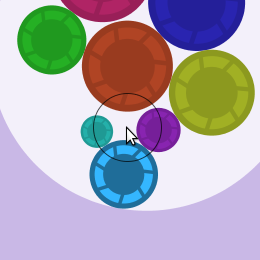
\includegraphics[scale=0.4]{drag}
\caption{The blue disk at the bottom is being dragged upward.
  A thin black outline around the mouse cursor indicates where
  the disk would be if it were not blocked by the others.}
\label{fig:drag}
\end{figure}

\begin{figure}
\centering
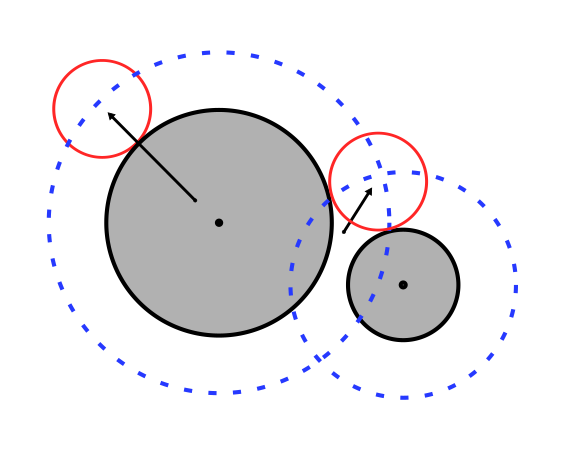
\includegraphics[scale=0.3]{expand}
\caption{Two disks (gray), their expanded boundaries
  (dashed blue), and two examples of shifts from overlapping
  positions to their closest valid positions.}
\label{fig:expand}
\end{figure}

\section{Disk Packing}

Our general approach is simply to iterate through the list
of disks, placing each disk into a valid position based on
some greedy heuristic.
We considered an {\it outward} strategy of placing each disk
in the position that results in the minimum increase in the
enclosing circle's radius, but experimentation pointed us
instead to a more effective  {\it inward} strategy of
starting at the perimeter of some enclosing circle and
working in toward the center.

The inward strategy requires knowing the radius of the
enclosing circle before placing any disks, and it may fail
if the radius is too small.
So we do many packing attempts with different circle sizes,
using a binary search to find the minimum radius such that
the packing algorithm succeeds.

\begin{algorithm}
\hrule\vspace{10pt}
\begin{program}
r_\text{min} \leftarrow \sqrt{\text{sum of disk areas} / \pi}
r_\text{max} \leftarrow \text{sum of disk radii}
P \leftarrow \bot
|while| \; r_\text{max} - r_\text{min} > \varepsilon
~~~~\tab%
  r \leftarrow \text{average}(r_\text{min}, r_\text{max})
  p \leftarrow \text{pack (Algorithm \ref{alg:pack}) with radius} \; r
  |if| \; \text{packing was successful}
  ~~~~\tab%
    r_\text{max} \leftarrow r
    P \leftarrow p
  \untab
  |else|
  ~~~~\tab%
    r_\text{min} \leftarrow r
  \untab
\untab
|return| \; P
\end{program}
\hrule
\caption{Radius selection}
\end{algorithm}

We found no reliable best way to choose the order in which
disks are placed, so we simply try various randomly-selected
permutations.

We search for candidate disk positions using the same
point and expanded-disk model used to deal with multi-disk
collisions, but in this case we also must respect the
constraint imposed by the enclosing circle.
This still easily fits within the model, however --
we simply need to {\it reduce} the enclosing circle's
radius rather than expand it.
We the position each disk by choosing the valid intersection
point farthest from the center of the enclosure.

\begin{algorithm}
\hrule\vspace{10pt}
\begin{program}
|repeat| \; 100 \; \text{times}
~~~\tab%
\text{randomly permute list of disks}
\text{position first disk arbitrarily at enclosing edge}
|for| \; \text{disk} \; d \; |in| \; \text{remaining disks}
~~~~\tab%
  B \; \leftarrow \; \tab [ \; \text{positioned disks expanded by} \; d\text{.radius}) \; ]
           + \; [ \; \text{enclosing circle reduced by} \; d\text{.radius} \; ] \untab
  I \leftarrow \{ i \in \cup_{(b_1, b_2) \in B^2} \; b_1 \cap b_2 : i \; \text{is valid} \}
  |if| \; I = \phi \; |then| \; |continue|
  d\text{.center} \leftarrow \arg\max_{i \in I} \; [ \; \text{distance}(i, \textrm{center}) \; ]
\untab
|return| \; \text{disk positions}
\untab
|return| \; \bot
\end{program}
\hrule
\caption{Disk packing}
\label{alg:pack}
\end{algorithm}

\section{References}

Bourke, Paul. \textit{Intersection of two circles}.
\url{http://paulbourke.net/geometry/2circle/}

\end{document}

